\documentclass[12pt,a4paper]{report}

\usepackage[utf8]{inputenc}
\usepackage[english]{babel}
\usepackage{amsmath}
\usepackage{amsfonts}
\usepackage{amssymb}

\usepackage{float}
\usepackage{graphicx}
\usepackage{hyperref}
\hypersetup{pdftitle={Neural Networks Project Report},pdfauthor={Matteo Di Stadio, Marco Carfora}}

\author{Matteo Di Stadio - 1794111\\Marco Carfora - 1794568}
\title{Neural Networks Project Report}
\date{}

\begin{document}

\maketitle

\tableofcontents



\chapter{Definition of the task}

\section{Image classification}
In this day and age the branches of artificial intelligence and machine learning hold steady the leadership of technological advancements and proposals, with one big problem standing on top of many others, computer vision. \\
At first glance it looks like an easy task, given that a human takes little to no effort telling two different things apart, like a cat from a dog, but that is thanks to the complex and marvelous structure of the human brain, which is very hard to feasibly replicate on hardware and software. The problem of computer vision is arguably one of the best to show this contrast, as it can still be tricky to this very day and many proposals were made across the years to find the best possible solution. The reason why we concentrate this hard on it is quite simple, as humans take action based on the study of their surroundings, whose important informations can be captured throught our senses, especially vision. What we mean with computer vision then is having the machine recognize the patterns of an object in order to discern what it can or is required to do in the given situation. A killer application can be found within automotive, as it is mandatory, in order to have a self-driving car, that the system is able to distinguish between the different road signals, the three traffic lights or between a passerby and a cyclist. This very problem can be taken back to probably the most important aspect of computer vision, the same we are exploring in this report, image classification. \\ \\
Considering this task then, a neural network would be the most adequate available technique, as the biggest problem with this duty is the difficulty in finding useful features. In fact, a neural network is able not only to learn a model for classification, but also to create and select autonomously useful features, instead of the manual process of creating them
from the images like shapes, edges or regions. 


\section{Convolutional neural networks}
Images can be seen as tensors, 3D tensors to be specific, with one dimension for the height of the pixels matrix, another one for its width and a final one for the RGB triple of each pixel. The best type of net to deal with these kinds of problems is then a convolutional neural network, where at least one of its hidden layers uses convolution, a mathematical operation which can be roughly described as a transformation of the input where every new element depends on a portion of the input itself and a separate kernel. A CNN can be divided in three stages:
\begin{itemize}
\item \textbf{Convolutional Stage}: when the convolution is applied. Its efficency in dealing with these kinds of problems is here seen thanks to its properties of sparce connectivity (the output depends on only a fraction of the input, given the smaller size of the kernel), parameter sharing (only a small shared set of parameters is learned from the kernel) and padding (a variable number of fictitious units added in order to be able to perform convolution even at the extremes of the input).
\item \textbf{Detector Stage}: the moment in which the non linear activation function is applied.
\item \textbf{Pooling Stage}: an aggregate function is applied to the previous output to shrink the results, so that it can focus on the key factors. The choice usually falls back to either max pooling (it returns the max value of the considered region) or average pooling (it returns the value average of the considered region).
\end{itemize}
Many CNN proposals were made throught the years in order to tackle this problem as is, but one big contribution in finding some of the best convolutional nets can be attributed to ImageNet. It is a large visual database designed for use in visual object recognition software research, where more than fourteen millions images have been hand-annotated by the project to indicate what objects are pictured, considering more than twenty thousand categories; many different networks still use it to train with great results. ImageNet is also responsible for the ImageNet Large Scale Visual Recognition Challenge (ILSVRC), which evaluates algorithms for object detection and image classification at large scale. One high level motivation is to allow researchers to compare progress in detection across a wider variety of objects, taking advantage of the quite expensive labeling effort, while another one is to measure the progress of computer vision for large scale image indexing for retrieval and annotation. \\
Many different methods came out of ILSVRC winners and runner-ups, all of which have various merits up their sleeve, including the one analyzed in this report, VGG (Visual Geometry Group), which ended up being the first runner-up of the ILSVRC competition in 2014.



\chapter{VGG method}

\section{Basic structure}
The VGG network architecture was described by Karen Simonyan and Andrew Zisserman in a paper written in 2014, called "Very Deep Convolutional Networks for Large Scale Image Recognition" \cite{VGGpaper}. \\
It has a very simple architecture, especially compared to the rather large receptive fields of its predecessors, as it uses only 3x3 convolutional layers (the smallest size matrix to identify left/right, up/down and center positions) throughout the whole net, with stride fixed to one pixel and the spatial padding of type "same", where the size of the padding is equal to half the kernel width in order to mantein constant dimension for each layer, preserving the spatial resolution after convolution. The volume size gets reduced by the max pooling layers which follow some of the convolutional ones and are performed over a 2x2 pixel window with stride two. At the end it also adds three fully connected layers, with the first two having 4096 channels each and the final one having 1000 of them. Given the context of multiclass classification, the problem better translates to a softmax output function for the hidden layers, a categorical cross entropy for the loss function and rectified linear units (ReLU) as activation functions. \\
For image recognition specifically, the input is fixed at size 224x224 and type RGB, with the only in house preprocessing done being the subtraction of the mean RGB value, computed on the training set, from each pixel. \\ \\
The VGG research group released a series of six possible convolutional network models, named A to E, all following the same basic structure described in the original paper, with the main difference being in their depths. They served the purpose of understanding how the depth of convolutional networks affects the accuracy of the models of large-scale image classification and recognition. \\
The minimum VGG11 has eight convolutional layers and three fully connected layers, compared to the maximum VGG19 which has sixteen convolutional layers and three fully connected layers. All the different variations are exactly the same in the last three fully connected layers, while the overall structure includes five sets of convolutional layers, followed by max pooling. As the depth increases, that is as we move from VGG11 to VGG19, what happens is that more and more cascaded convolutional layers are added in those five sets. Based on experimental and practical results, the most famous and used variants, that we are going to explore in this report, are the 16 one and the 19 one. \\
While its depth and fully connected nodes may bring up some cons in using the VGG architecture, namely it being slow to train and with quite large weights, it is still considered a strongly valid candidate to use in this context, since its accuracy and loss held for a very long time the best position among image classifiers and it holds up pretty well even by today standards, especially thanks to its lower complexity in comparison to other state of the art structures.
\begin{figure}[H]
\centering
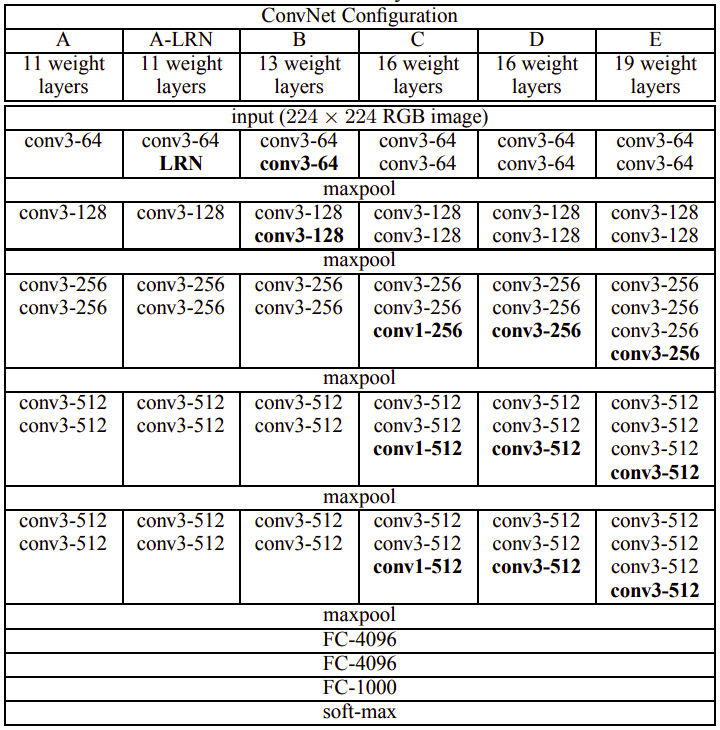
\includegraphics[scale=0.4]{./immagini/vgg_layers_table.png}
\caption{\textit{This table indicates the A-E VGG configurations from the paper \cite{VGG_configurations_table}}}
\label{fig:vgg_layers_table}
\end{figure}


\section{VGG16 and VGG19}
Like we mentioned above, both VGG16 and VGG19 share the same general structure, with their inputs consisting of RGB images of size 244x244, which get passed through a stack of convolutional layers one after another, where the used filters have a very small receptive field of 3x3, strinde of one pixel and "same" padding. The pooling is carried out by the five homonymous layers set after the five blocks of convolution, with a 2x2 pixel window and stride two. After all of that, as stated before, three fully connected layers are also added. \\ \\
The main differences from one another lie in the  weighted layers number, as while VGG16 has a total of 41 layers (13 of which are convolutional ones and the other nominal 3 are from the fully connected base) the VGG19 on the other hand adds six new layers, three of which are weighted ones, for a total of 16 and 19 as their names implies. Another difference then is in filter size, with the general number being between 64 and 128 in VGG16 and between 256 and 512 in VGG19. On top of that, VGG16 uses the ReLU five times, while the VGG19 up to eighteen times.
\begin{figure}[H]
\centering
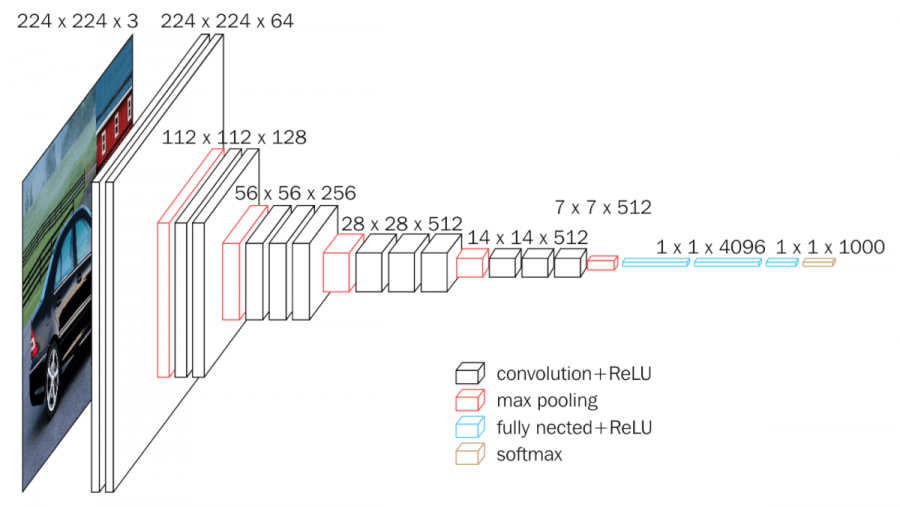
\includegraphics[scale=0.3]{./immagini/vgg16_structure.png}
\caption{\textit{VGG16 structure \cite{VGG16_image}}}
\label{fig:vgg16_structure}
\end{figure}
\begin{figure}[H]
\centering
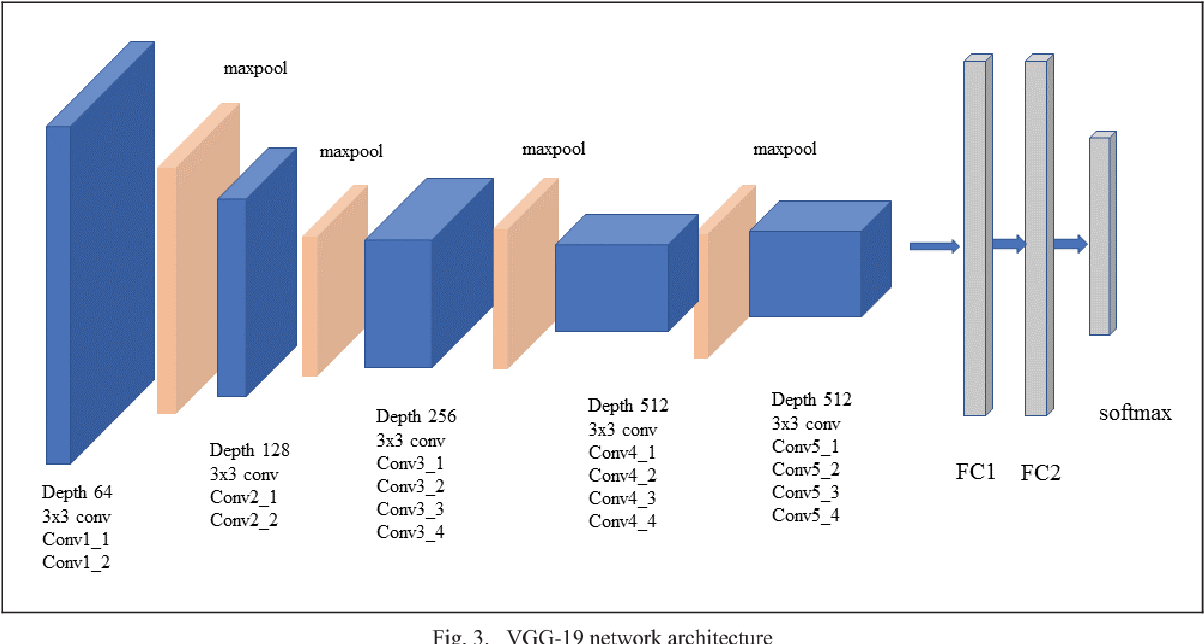
\includegraphics[scale=0.3]{./immagini/vgg19_structure.png}
\caption{\textit{VGG19 structure \cite{VGG19_image}}}
\label{fig:vgg19_structure}
\end{figure}



\chapter{Experimentations}

\section{General informations}
Having defined the methods and its models to use inside this project, before throwing ourself headlong we must establish the 
dataset to use. There are many different captivating image classification tasks that we could have used, but one particular dataset caught our interest. It was a set of 4774 photos from 20 classes captured by the ARGOS system \cite{argos_dataset}, operating 24/7 in the city of Venice (Italy). It is quite a unique dataset, coming from an incomparable environment like Venice, which can actually be of great help in the problem of the tracking and classification of people and vehicles, a fundamental processes in intelligent surveillance systems, thanks to the challenges that it brings to the table, due to the changes in the environmental conditions (like for example boat wakes, waves or reflections), meaning that robust techniques, validated through the ARGOS boat classification dataset, will improve the development and deployment of solutions in similar applications related to vehicle detection and classification. \\
Moving on the practical side, the aforementioned dataset was placed inside a Google Drive folder, so that it could be easily retrieved later on by the code. Before that though, another step had to be done, an indispensable one to the process as a whole. In fact, one big problem of machine learning is the dangerous overfitting, that can also surface in the presence of peculiar datasets, where, for instance, erroneous values can cause the training to end up too much taylor made for the informations at hand. In order to try to prevent this, it is highly suggested to split the dataset up in a training set, used during the homonymous session, and a validation set, used later on to test the validity of the trained model. It is still prefarable to have the majority of the data inside the training set (with a minimum cardinality of at least thirty elements), in order to end up with a better training, but it is also better to not have a small set of test data, so a trade off has to be found, like, for istance, reserving roughly one third of the dataset to the testing set. While this was an important step to do, several classes, which already suffered from lack of images, ended up with an even smaller group of images per set, a problem that will be touched upon later on. \\ \\
After the splitting of the dataset we moved on to Python 3, the coding language that was used for this report, as it offers a vast repertoire of neural networks notions. More specifically, we used the Keras module, a library which brings the TensorFlow environment to Python, easing the process of importing fondamental constructs that were later used during the experiments. \\
Before starting the coding itself though, having to train the net using several different parameters and strategies we needed to define a way to compare them all and choose the best options overall. We had to define some evaluation techniques of the performance according to the common metrics used in neural networks. The following definitions represent the metrics that were used in the end:
\begin{itemize}
\item \textbf{Accuracy}: the most intuitive performance measure, as it is simply a ratio of correctly predicted observation to the total observations. The more it grows the better. However, accuracy is a great measure only in presence of symmetric datasets where values of false positive and false negatives are almost the same.
\item \textbf{Loss}: it is defined as the difference between the predicted values by our model and the true values, so that the smaller the gap and the value are the better. The loss is computed on training and validation and it is linked to the behavior the model is having in these two sets, as it is the sum of errors made for each example in both of them.
\item \textbf{Precision}: the ratio of correctly predicted positive observations to the total predicted positive observations. It allows to see the false positives. The more it tends to one the better.
\item \textbf{Recall}: the ratio of correctly predicted positive observations to the all observations in actual class. It allows to see the false negatives. The more it tends to one the better.
\item \textbf{F1-Score}: the weighted average of precision and recall. It takes both false positives and false negatives into account, definitely more useful than accuracy, especially in the case of an uneven class distribution.
\item \textbf{Confusion Matrix}: considering the matrix itself CM, a row R and a column C, a confusion matrix replenishes itself by filling in the CM[R][C] position the number of instances of class R that where collocated in class C. Because of that, the more the main diagonal is filled the better.
\end{itemize}


\section{VGG16 experiments}
The first model that we tried was the 16 weighted layers one, which was actually the one used in the ILSVRC 2014 and it is still considered one of the best uses of this method. The first step was to retrieve the images inside the respective training and testing sets, with color mode RGB and target size of 224x224, the standards for VGG. With that out of the way, it was time to construct the actual model from scratch, following the specifics that have been described up to this point. \\
At first a sequential model was initialized, so that it can group a linear stack of layers into a Keras model and provide training and inference features on it. Then the first block was added, composed by two convolutional layers and a max pooling one, all following the specifications of VGG, like a kernel size of 3x3, a ReLU activation function and padding of type "same". Then after that the remaining four blocks were added, respectively the second one composed by two convolutional layers and one max pooling and the other three composed by three convolutional layers and one max pooling. After flattening the result, the first dense layer was created using again a ReLU activation function. A second one was created the same way, while the third and last one was given a softmax output function due to the multiclass classification problem. \\
The final step was to compile the model with Keras in order to be used for training later on. A categorical cross entropy loss function was assigned and an Adam optimizer was specified with a standard suggested learning rate of 0.0001. Adam (whose name is based on "adaptive moment estimation") is an optimization algorithm that can be used instead of the classical stochastic gradient descent procedure to update network weights iteratively based in training data. Among its benefits there are a straightforward implementation, efficency, little memory requirements and above all else it is well suited for problems that are large in terms of data and parameters, like an image classification one. Adam is different to classical stochastic gradient descent because while they mantein a single learning rate for all weight updates that does not change during training, it uses a learning rate for each parameter that is separately adapted as the learning unfolds, all thanks to the estimations of the first and second moments of the gradients. Having said all of that, plus the fact that empirical results demonstrate the effectiveness of Adam over other available stochastic optimization methods, it was decided to adoperate it as our optimizer. \\
At this point it was possible to proceed with the training itself, setting a maximum of 30 epochs and implementing an Early Stopping callback technique. Since the training is the most time and resource consuming part of the whole process, Keras allows to stop it before the epochs actually terminate through this callback if it senses that the process is deteriorating or not improving in some meaningful way. Given the nature of these early experiments we decided to have it monitoring that the validation accuracy is not degrading and with a suggested value of patience 3, meaning that is the number of epochs with no improvement after which training will be stopped. After the training was done, the results were evaluated using the aforementioned metrics:
\begin{figure}[H]
\centering
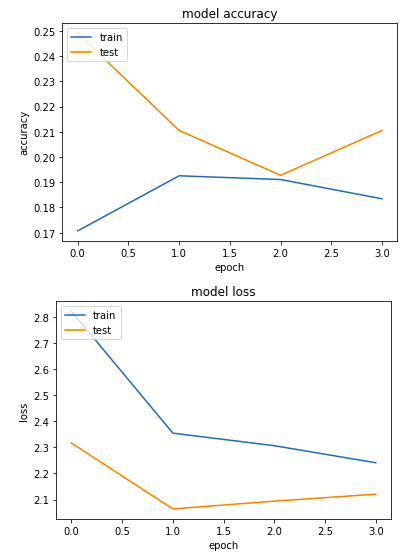
\includegraphics[scale=0.4]{./immagini/vgg16/0_data_augmentation_-_3_patience_stopping_-_no_dropout_-_no_batch_norm/plot_loss_accuracy.png}
\caption{\textit{The plots of accuracy and loss using VGG16 as described before.}}
\end{figure}
\begin{figure}[H]
\centering
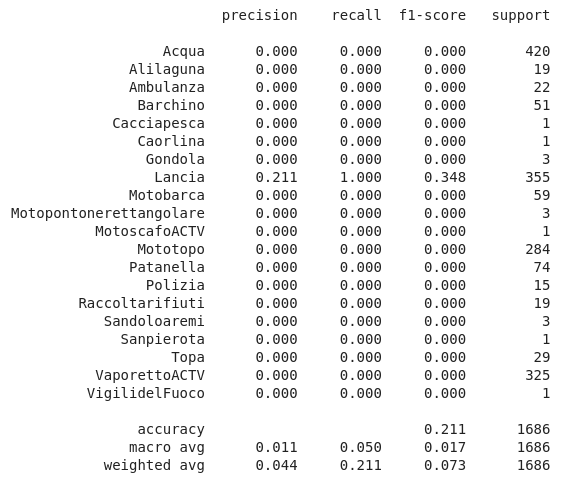
\includegraphics[scale=0.4]{./immagini/vgg16/0_data_augmentation_-_3_patience_stopping_-_no_dropout_-_no_batch_norm/f1.png}
\caption{\textit{The precision, recall and F1-score using VGG16 as described before.}}
\end{figure}
\begin{figure}[H]
\centering
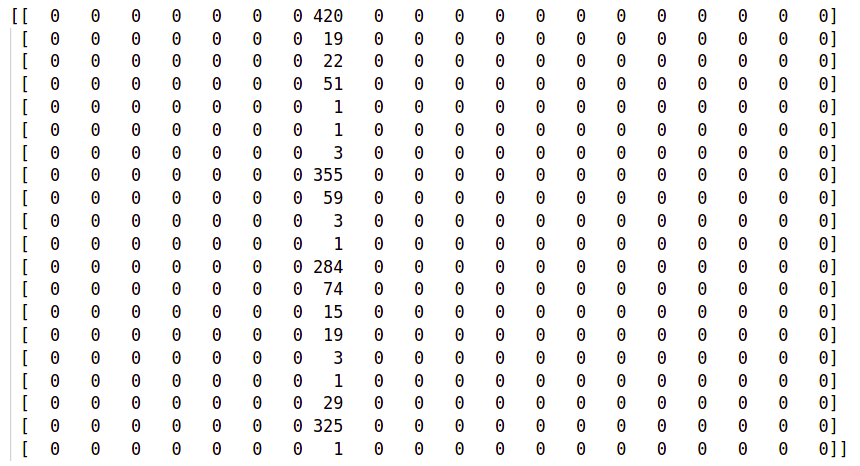
\includegraphics[scale=0.4]{./immagini/vgg16/0_data_augmentation_-_3_patience_stopping_-_no_dropout_-_no_batch_norm/cm_num.png}
\caption{\textit{The confusion matrix using VGG16 as described before.}}
\end{figure}

The results of this first experiment are lackluster to say the least. The accuracy was abysmally small, both in training and in validation, while the loss was not very great either, with a bad tendency to go even higher. Fortunately the Early Stopping managed to arrest the training preventively, as it clearly needed, as expected, some more adjustments. This terrible result is even more exemplified by taking a look at the values of F1-score and the corresponding confusion matrix, where all the testing samples are erroneously grouped under one single class. \\
Before in the report we mentioned how several classes in the dataset suffered from lack of images, and the important division between training and testing sets exacerbated it even more. This thing, which may seem like a little inconvenience at first glance, is actually the big problem that led to these terrible results. A small dataset, especially on the training side, in prone to negatively affect the fitting. With that being the problem then the solution is to amplify the set, which is not exactly as immediate as it may sound, as the problem of finding more labeled samples has always been a big one. To compensate it was then introduced the concept of data augmentation \cite{data_augmentation}, meaning that for each image in the training set an accurately distorted clone can be created by rotating, translating, zooming in or out, color inverting or shifting and
flipping in all four directions the original picture. This simple solution can greatly help in avoiding overfitting or underfitting and must be done as soon as possible, before the definition and training of the model, otherwise results like the ones we just saw are to be expected. \\
As a matter of fact, the images that follow are the results of the exact same process as before but with the addition of a good level of data augmentation. While some classes still cause little problems, these numbers are definitely more acceptable. The accuracy and loss functions are closer to their testing counterparts, which now have a good expected trend, while the F1-scores and the structure of the confusion matrix are way more reassuring.
\begin{figure}[H]
\centering
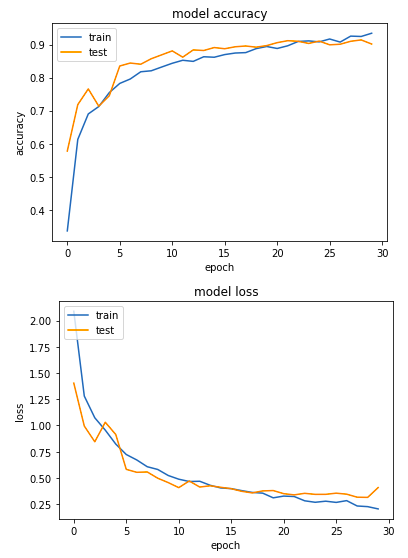
\includegraphics[scale=0.4]{./immagini/vgg16/2_data_augmentation_-_30_epochs_no_stopping_-_no_dropout_-_no_batch_norm/plot_loss_accuracy.png}
\caption{\textit{The plots of accuracy and loss using VGG16 after the addition of data augmentation.}}
\end{figure}
\begin{figure}[H]
\centering
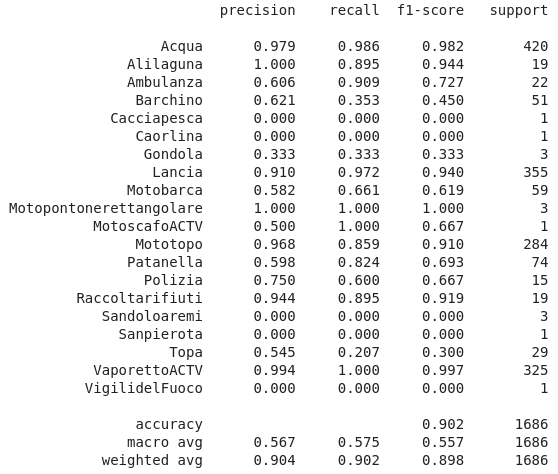
\includegraphics[scale=0.4]{./immagini/vgg16/2_data_augmentation_-_30_epochs_no_stopping_-_no_dropout_-_no_batch_norm/f1.png}
\caption{\textit{The precision, recall and F1-score using VGG16 after the addition of data augmentation.}}
\end{figure}
\begin{figure}[H]
\centering
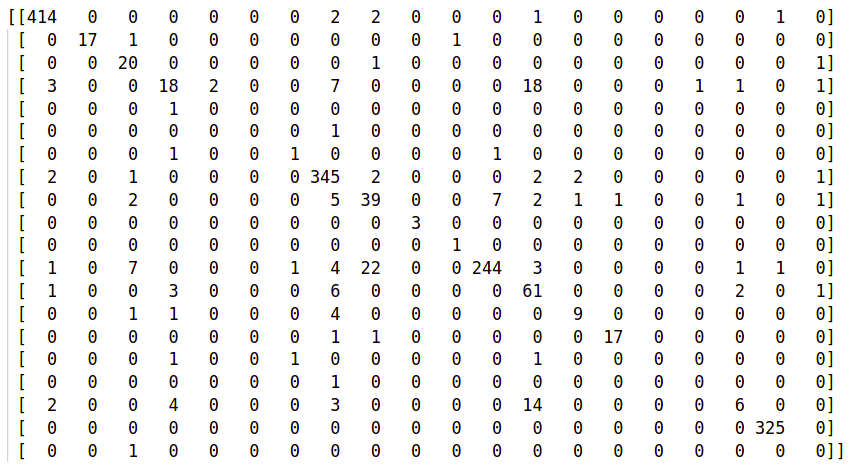
\includegraphics[scale=0.4]{./immagini/vgg16/2_data_augmentation_-_30_epochs_no_stopping_-_no_dropout_-_no_batch_norm/cm_num.png}
\caption{\textit{The confusion matrix using VGG16 after the addition of data augmentation.}}
\end{figure}

Staring at these last results, it is clear that more optimizations are possible to get even better outcomes. One addition can be in the form of Dropout \cite{dropout}, which offers a very computationally cheap and remarkably effective regularization method to reduce overfitting and improve generalization error in deep neural networks of all kinds. The basic idea is that it approximates training a large number of neural networks with different architectures in parallel. During training, some number of layer outputs are randomly dropped out (temporarily removed from the net, along with all its incoming and outgoing connections), with the effect of making the layer look like and be treated like a layer with a different number of nodes and connectivity to the prior one. This is done in order to mitigate overfitting and the likes with the smallest possible computational expense, as a single model can be used to simulate having a large number of different network architectures by randomly dropping out nodes during training. \\
Keras makes available Dropout for these kinds of models, setting up a rate signifying the frequency at which the layers randomly set the input units to 0 at each traing step (while no values are dropped during inference); the inputs that are not set to 0 are instead scaled up by 1/(1 - rate) such that the sum over all inputs is unchanged. Having said that, two dropout layers were added to the first two dense fully connected ones, as it seemed like the best spot to apply such regularization, and in fact, comparing the results gained from adding this last optimization to the latest structure we can see a great improvement. The trends of the validation accuracy and validation loss follow the expected course, never being too far from the training ones, not to mention that the numbers of the confusion matrix and the F1-scores validates even more the outcomes, with only those classes that are still heavily affected by the division between training and testing sets giving little to no problems.
\begin{figure}[H]
\centering
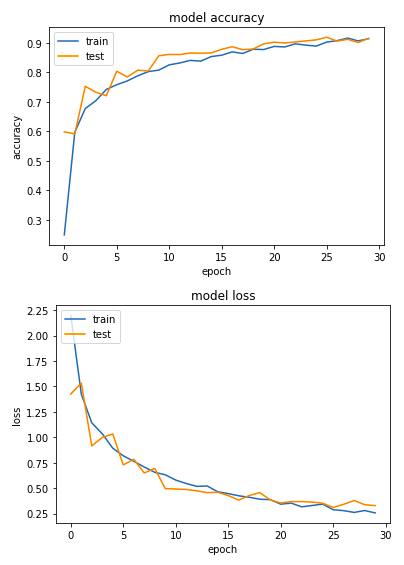
\includegraphics[scale=0.4]{./immagini/vgg16/2_data_augmentation_-_30_epochs_no_stopping_-_dropout_0p5_-_no_batch_norm/plot_loss_accuracy.png}
\caption{\textit{The plots of accuracy and loss using VGG16 after the addition of Dropout.}}
\end{figure}
\begin{figure}[H]
\centering
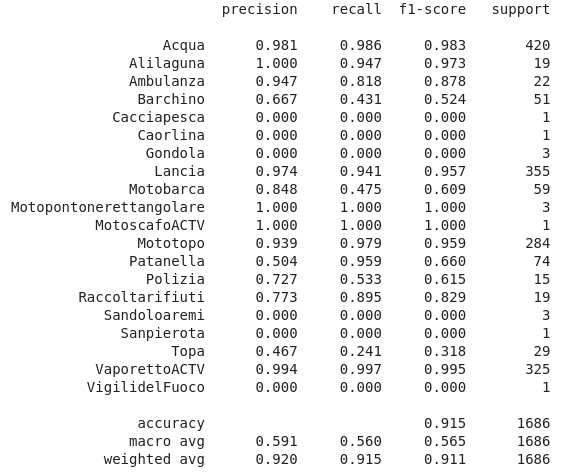
\includegraphics[scale=0.4]{./immagini/vgg16/2_data_augmentation_-_30_epochs_no_stopping_-_dropout_0p5_-_no_batch_norm/f1.png}
\caption{\textit{The precision, recall and F1-score using VGG16 after the addition of Dropout.}}
\end{figure}
\begin{figure}[H]
\centering
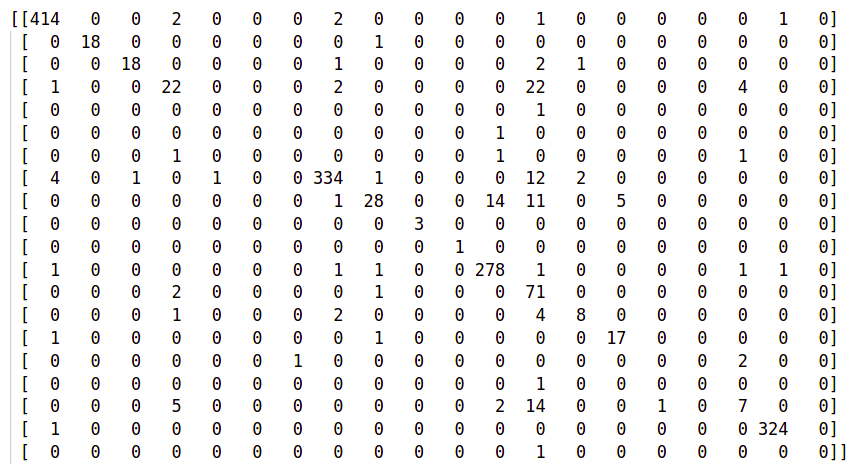
\includegraphics[scale=0.4]{./immagini/vgg16/2_data_augmentation_-_30_epochs_no_stopping_-_dropout_0p5_-_no_batch_norm/cm_num.png}
\caption{\textit{The confusion matrix using VGG16 after the addition of Dropout.}}
\end{figure}

While these latest results are almost flawless, one can beg the question if something more can still be applied. Among other regularization methods there is Batch Normalization \cite{batch_normalization}. This type of normalization was actually invented after the first 
definition of the VGG method, so it was absent from its standard formulation, but this has not stopped several takes at implementing them both together. In general, training deep neural networks with tens of layers is challenging as they can be sensitive to the initial random weights and configuration of the learning algorithm. One possible reason for this difficulty is attributed to the distribution of the inputs to layers deep in the network that may change after each mini batch when the weights are updated, a process that is called internal covariate shift. Batch Normalization is then a technique for training very deep neural networks that standardizes the inputs to a layer for each mini batch. This has the effect of stabilizing the learning task and dramatically reducing the number of training epochs required to train deep networks. \\
Various studies are still going on about the best way to implement it, like for instance where to put it best or if it actually conflicts with Dropout or not, but trying it out may be worth the effort. So, we added a couple of Batch Normalization layers inside the first two dense blocks of the fully connected net below, as initially suggested, and let it train for 30 epochs. The corresponding results are promising, with the exception of that final spike in the accuracy and loss plots the trends are not bad and the numbers given by the confusion matrix and the F1-scores are comparable and in some cases even better than what we managed to find before. Using some kind of Early Stopping would probably end the training sooner, that would also improve the final values, which definitely would be consistent with what we can see now and what we expected to see.
\begin{figure}[H]
\centering
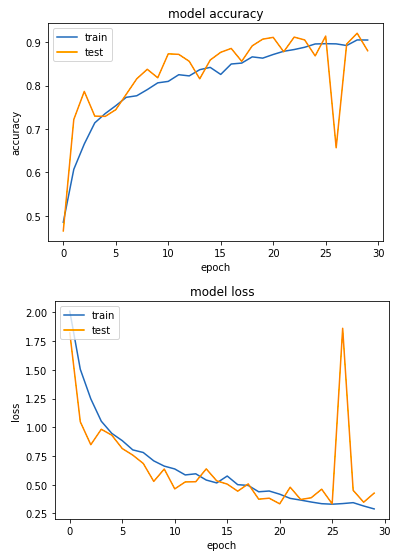
\includegraphics[scale=0.4]{./immagini/vgg16/2_data_augmentation_-_30_epochs_no_stopping_-_dropout_0p5_-_classifier_batch_norm/plot_loss_accuracy.png}
\caption{\textit{The plots of accuracy and loss using VGG16 after the addition of Batch Normalization.}}
\end{figure}
\begin{figure}[H]
\centering
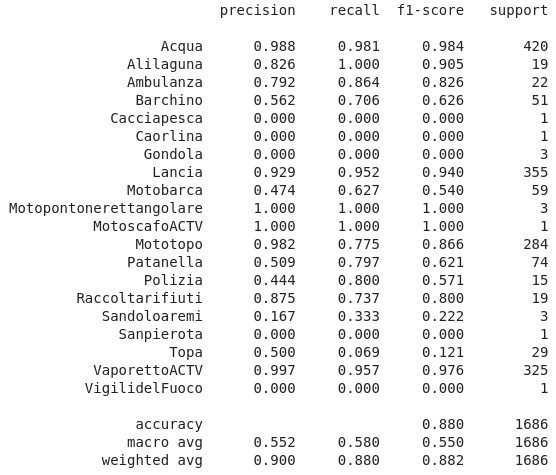
\includegraphics[scale=0.4]{./immagini/vgg16/2_data_augmentation_-_30_epochs_no_stopping_-_dropout_0p5_-_classifier_batch_norm/f1.png}
\caption{\textit{The precision, recall and F1-score using VGG16 after the addition of Batch Normalization.}}
\end{figure}
\begin{figure}[H]
\centering
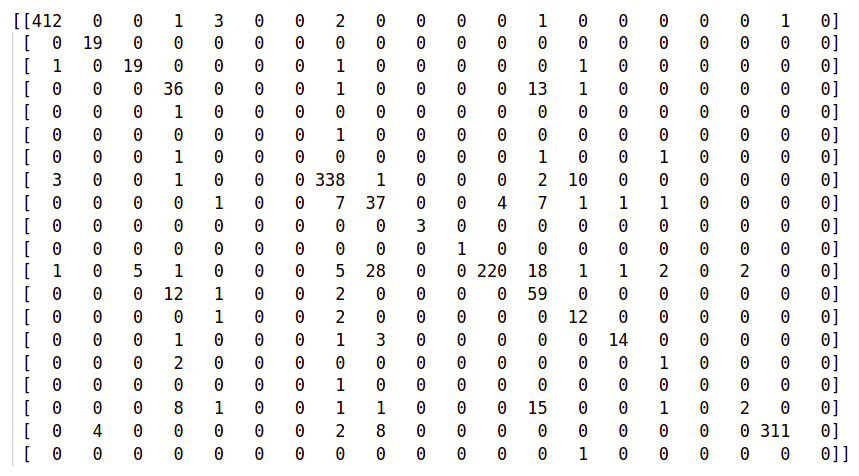
\includegraphics[scale=0.4]{./immagini/vgg16/2_data_augmentation_-_30_epochs_no_stopping_-_dropout_0p5_-_classifier_batch_norm/cm_num.png}
\caption{\textit{The confusion matrix using VGG16 after the addition of Batch Normalization.}}
\end{figure}



\section{VGG19 experiments}
In this section we observe the experiments executed with the VGG19 model instead. The modalities are almost similar to the ones we already saw in the previous section. We will see again the importance of data augmentation given the datasaet used inside this report; how the Early Stopping callback can help us cutting out unnecessary training (even if it didin't arrive to the last epoch) which would waste precious time and resources; how the Dropout regularization (which we decided to have already implemented from the start inside the following experiments given the great results it gave us previously) gave us a great boost in performance and accuracy and how the Batch Normalization could improve the overall trends of the results if correctly applied. Having said all of that, here it is a list of the VGG19 experiments with the corresponding parameters. \\ \\
At the beginning we start implementing the most easy and standard configuration of the network, just like with VGG16, without using data augmentation, in order to better show how it still is crucially important even with an overall better model. We still keep Early Stopping with patience 3 in order to not waste too much time on this experiment, since we are pretty confident it will give us not so great results. As expected, the plots of the accuracy and loss are deteriorating, while just like in the VGG16 case the confusion matrix shows the worst possible results we could expect, as every single prediction came from one lone class, and very much the same happen in relation to the F1-scores, as we can see in the images below.
\begin{figure}[H]
\centering
\includegraphics[scale=0.45]{./immagini/vgg19/0_data_augmentation_-_3_patience_stopping_-_dropout_0p5_-_no_batch_norm/plot1.png}
\caption{\textit{The plot of accuracy using VGG19 as described before.}}
\end{figure}
\begin{figure}[H]
\centering
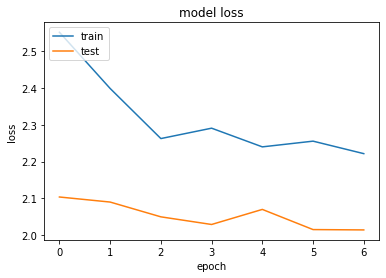
\includegraphics[scale=0.45]{./immagini/vgg19/0_data_augmentation_-_3_patience_stopping_-_dropout_0p5_-_no_batch_norm/plot2.png}
\caption{\textit{The plot of loss using VGG19 as described before.}}
\end{figure}
\begin{figure}[H]
\centering
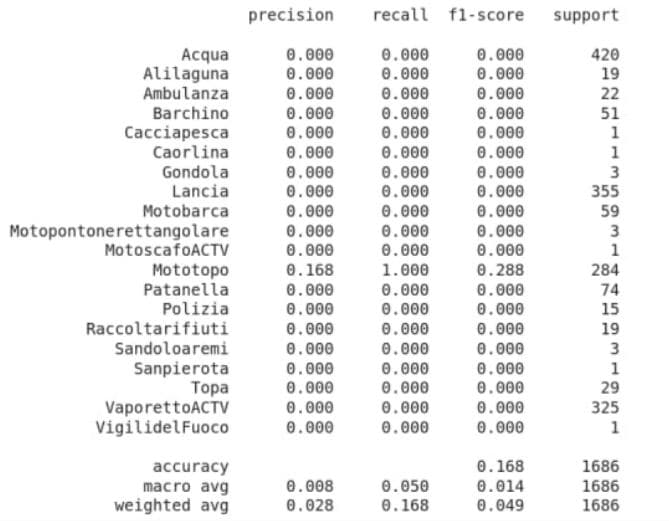
\includegraphics[scale=0.7]{./immagini/vgg19/0_data_augmentation_-_3_patience_stopping_-_dropout_0p5_-_no_batch_norm/f1.JPEG}
\caption{\textit{The precision, recall and F1-score using VGG19 as described before.}}
\end{figure}
\begin{figure}[H]
\centering
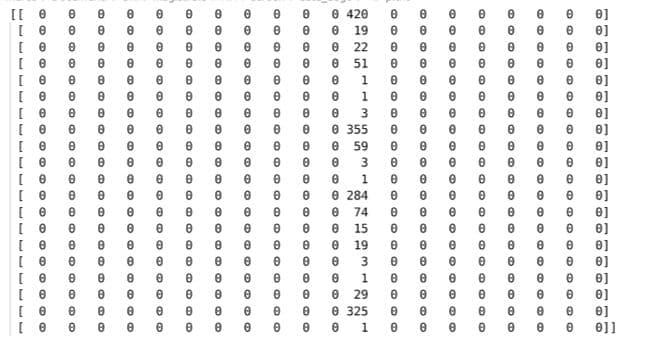
\includegraphics[scale=0.8]{./immagini/vgg19/0_data_augmentation_-_3_patience_stopping_-_dropout_0p5_-_no_batch_norm/cm_num.JPEG}
\caption{\textit{The confusion matrix using VGG19 as described before.}}
\end{figure}

Just like what we did with VGG16 we now added a good level of data augmentation in order to gain better results, which, as expected, actually arrived after this change. The images that follow are the results of the exact same process as before but with the addition of a good level of data augmentation. While some classes still cause little problems, these numbers are definitely more acceptable. The accuracy and loss functions are closer to their testing counterparts, which now have a good expected trend, while the F1-scores and the structure of the confusion matrix are way more reassuring.
\begin{figure}[H]
\centering
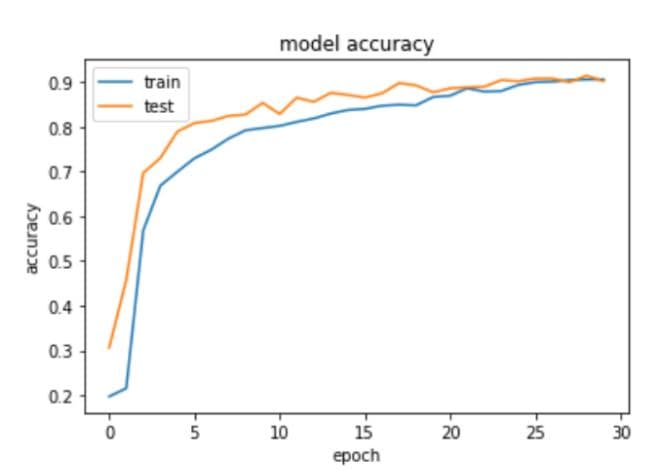
\includegraphics[scale=0.45]{./immagini/vgg19/2_data_augmentation_-_30_epochs_no_stopping_-_dropout_0p5_-_no_batch_norm/plot1.JPEG}
\caption{\textit{The plot of accuracy using VGG19 after the addition of data augmentation.}}
\end{figure}
\begin{figure}[H]
\centering
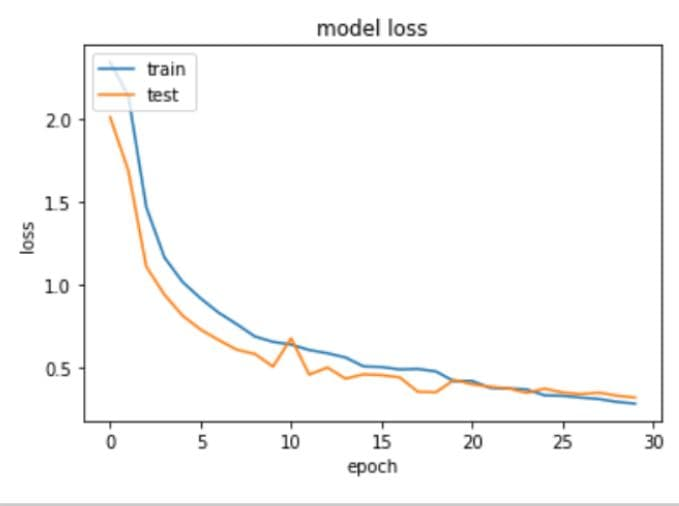
\includegraphics[scale=0.45]{./immagini/vgg19/2_data_augmentation_-_30_epochs_no_stopping_-_dropout_0p5_-_no_batch_norm/plot2.JPEG}
\caption{\textit{The plot of loss using VGG19 after the addition of data augmentation.}}
\end{figure}
\begin{figure}[H]
\centering
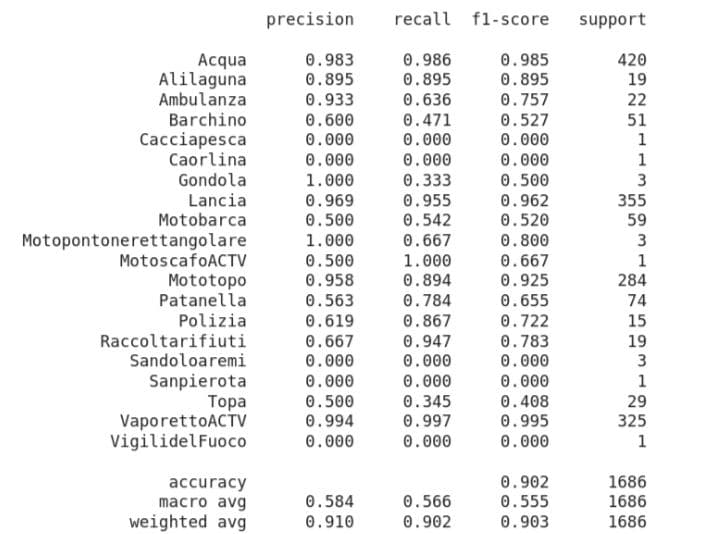
\includegraphics[scale=0.7]{./immagini/vgg19/2_data_augmentation_-_30_epochs_no_stopping_-_dropout_0p5_-_no_batch_norm/f1.JPEG}
\caption{\textit{The precision, recall and F1-score using VGG19 after the addition of data augmentation.}}
\end{figure}
\begin{figure}[H]
\centering
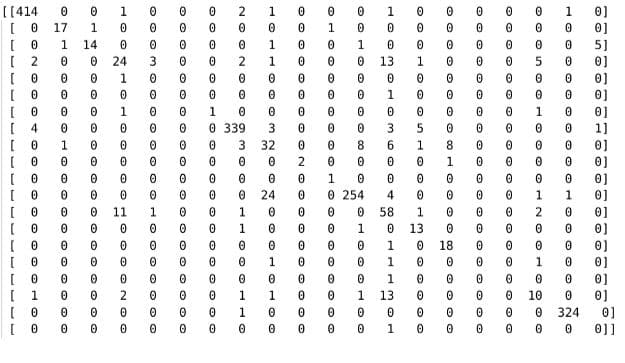
\includegraphics[scale=0.8]{./immagini/vgg19/2_data_augmentation_-_30_epochs_no_stopping_-_dropout_0p5_-_no_batch_norm/cm_num.JPEG}
\caption{\textit{The confusion matrix using VGG19 after the addition of data augmentation.}}
\end{figure}

Just like with VGG16 we then tried to unite the VGG method with the Batch Normalization, a thing that was not present in the standard as the latter was proposed after the initial creation of VGG. As always, we provide the same specifics as before, with the only difference being to put them on top of the 19 layers structure instead of the 16 layers one. \\
While in the VGG16 model this addition was a good one, it was not that far off the results of the Dropout addition, while here we can see that Batch Normalization finds itself really confortable if paired with VGG19. These results below are actually the best we have gotten, with a validation accuracy surpassing the training one, a miniscule validation loss which is almost equal to the training one, great values of F1-score even in some of the problematic classes and in the confusion matrix it is clearly possible to see the predictions falling back to the principal diagonal, as they should.
\begin{figure}[H]
\centering
\includegraphics[scale=0.45]{./immagini/vgg19/2_data_augmentation_-_30_epochs_no_stopping_-_dropout_0p5_-_classifier_batch_norm/plot1.png}
\caption{\textit{The plot of accuracy using VGG19 after the addition of Batch Normalization.}}
\end{figure}
\begin{figure}[H]
\centering
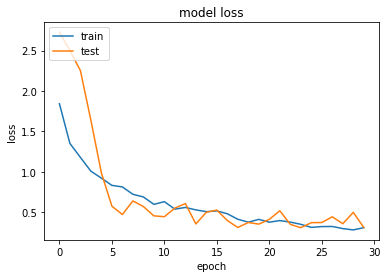
\includegraphics[scale=0.45]{./immagini/vgg19/2_data_augmentation_-_30_epochs_no_stopping_-_dropout_0p5_-_classifier_batch_norm/plot2.png}
\caption{\textit{The plot of loss using VGG19 after the addition of Batch Normalization.}}
\end{figure}
\begin{figure}[H]
\centering
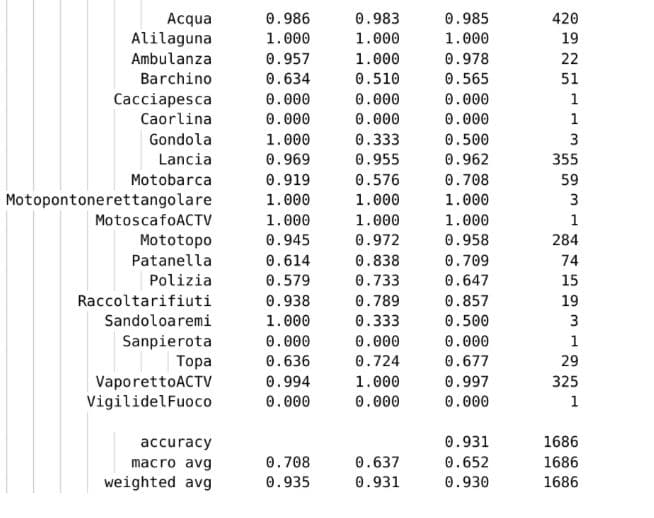
\includegraphics[scale=0.7]{./immagini/vgg19/2_data_augmentation_-_30_epochs_no_stopping_-_dropout_0p5_-_classifier_batch_norm/f1.JPEG}
\caption{\textit{The precision, recall and F1-score using VGG19 after the addition of Batch Normalization.}}
\end{figure}
\begin{figure}[H]
\centering
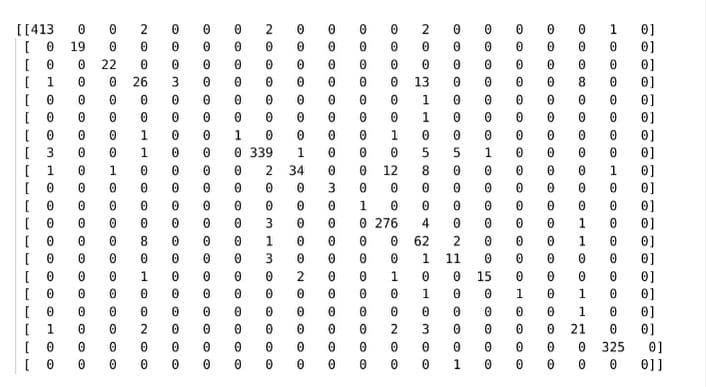
\includegraphics[scale=0.8]{./immagini/vgg19/2_data_augmentation_-_30_epochs_no_stopping_-_dropout_0p5_-_classifier_batch_norm/cm_num.JPEG}
\caption{\textit{The confusion matrix using VGG19 after the addition of Batch Normalization.}}
\end{figure}

\pagebreak

This experiment marks the end of our studies. We managed to find very interestings results which gave us a better perspective to how to best tackle the computer vision problem using the VGG method. VGG16 is still widly used, and rightfully so, as with the right conditions it can perform really well, while VGG19, being the most articulate of the six VGG configurations, presents the best overall outcomes considering the same initial conditions and is able to better work together with Batch Normalization, an newer optimization that we can say has a promising relationship with this model in this particular environment. This report also managed to highlight the importance of data augmentation and having big and variegated datasets, as if we would have stopped at face value we would have not discovered the great potential of this network in the image classification context. Furthermore, we also saw how we can usefully implement other kinds of optimizers and tricks like Adam, Dropout and the Early Stopping callback, so that the process can procede smoothly and with better overall findings.



\begin{thebibliography}{1}
\bibitem{VGGpaper}
Original VGG paper:\\https://arxiv.org/pdf/1409.1556.pdf
\bibitem{VGG_configurations_table}
VGG configurations table image source:\\https://arxiv.org/pdf/1409.1556v6.pdf
\bibitem{VGG16_image}
VGG16 image source:\\https://neurohive.io/wp-content/uploads/2018/11/vgg16-1-e1542731207177.png
\bibitem{VGG19_image}
VGG19 image source:\\https://miro.medium.com/max/2400/1*6U9FJ{\_}se7SIuFKJRyPMHuA.png
\bibitem{argos_dataset}
Paper about the Argos dataset:\\https://www.researchgate.net/publication/309630436{\_}ARGOS-Venice{\_}Boat{\_}Classification
\bibitem{data_augmentation}
Paper about data augmentation:\\www.researchgate.net/publication/325920702{\_}Data{\_}augmentation{\_}for{\_}\\improving{\_}deep{\_}learning{\_}in{\_}image{\_}classification{\_}problem
\bibitem{dropout}
Paper about Dropout:\\https://jmlr.org/papers/volume15/srivastava14a/srivastava14a.pdf
\bibitem{batch_normalization}
Paper about Batch Normalization:\\https://arxiv.org/pdf/1502.03167v3.pdf
\end{thebibliography}



\end{document}
